\section{时间序列中的规模效应}
\label{sec:renewal}

前两节假定上一代感染者人数 $n$ 已知。真实监测序列不满足这一点。下一周的新感染由此前几周的感染共同产生，感染压力可写为 $\Lambda_{t+1}=\sum_{s\geq1}w_sI_{t+1-s}$，其中 $w_s$ 是世代间隔分布。漏报使 $I_1,\dots,I_t$ 无法完全观测，所以下一周的感染压力 $\Lambda_{t+1}$ 也是随机的。实际能用的只是报告数的加权和 $D_t=\sum_{s\geq1}w_sC_{t+1-s}$，并以 $G_t=C_{t+1}/D_t$ 作为增长统计量。

\subsection{信息集与误差分解}
\label{sec:renewal-decomp}

预测误差取决于可用的信息集。记 $\mathcal F_t$ 为截至第 $t$ 周的全部报告，$m=\rho\,\E(\Lambda_{t+1}\mid\mathcal F_t)$。

\begin{remark}
\label{rem:information}
设给定 $\Lambda_{t+1}$ 与 $R_{t+1}$ 时，$C_{t+1}$ 服从式~\eqref{eq:report-dist} 中以 $\Lambda_{t+1}$ 代替 $n$ 的负二项分布，且在 $\mathcal F_t$ 条件下 $\Lambda_{t+1}$ 与 $R_{t+1}$ 独立。两次使用全方差公式，可得
\begin{equation}
  \frac{\Var(C_{t+1}\mid\mathcal F_t)}{[\rho\,\E(\Lambda_{t+1}\mid\mathcal F_t)]^2}
  =v_R+\frac{A}{m}+\CV^2(\Lambda_{t+1}\mid\mathcal F_t)\,(\Rbar^2+v_R).
  \label{eq:info-decomp}
\end{equation}
当 $\Lambda_{t+1}$ 完全已知时，变异系数项为零，式~\eqref{eq:info-decomp} 退化为命题~\ref{prop:average}。
\end{remark}

式~\eqref{eq:info-decomp} 中多出的一项来自感染压力的不确定性。它与规模无关，并会随漏报程度和世代间隔的展宽而变大。

实证中使用的误差指标有两种读法。用 $\Rbar D_t$ 预测 $C_{t+1}$ 的相对误差，与用 $G_t$ 估计 $\Rbar$ 的相对误差恒等
\begin{equation}
  \frac{(C_{t+1}-\Rbar D_t)^2}{(\Rbar D_t)^2}=\frac{(G_t-\Rbar)^2}{\Rbar^2}.
  \label{eq:identity}
\end{equation}
记 $\mu_t=\E(C_{t+1}\mid\mathcal F_t)$，$\sigma_t^2=\Var(C_{t+1}\mid\mathcal F_t)$。由于 $D_t$ 由 $\mathcal F_t$ 决定，增长统计量的均方误差可以分解为
\begin{equation}
  \E[(G_t-\Rbar)^2]=\E((\sigma_t/D_t)^2)+\E[(\mu_t/D_t-\Rbar)^2].
  \label{eq:mse-decomp}
\end{equation}
第二项是条件偏差，非负。第一项则不必等于 $v_R+A/D_t$，因为 $D_t$ 只是 $\rho\Lambda_{t+1}$ 的带噪代理，$(\sigma_t/D_t)^2$ 可能高于也可能低于单代公式。因此，单代公式 $(v_R+A/m)/\Rbar^2$ 在时间序列中只能作参照曲线，一般情况下不构成下界。

\subsection{更新过程仿真}
\label{sec:renewal-sim}

为了解参照曲线的偏离程度，我们模拟了带环境波动的更新过程。世代间隔取 4 周离散核，权重依次为 0.45、0.35、0.15、0.05；每周 $R_t$ 独立抽自均值 1.15、方差 0.04 的 Gamma 分布；$I_t\sim\NB(k\Lambda_t,\,k/(k+R_t))$，$k=0.35$；报告数 $C_t\sim\Bin(I_t,0.25)$。为避免轨迹灭绝，$I_t$ 截断为不小于 1。前 4 周的感染数设为 $m_0/\rho$，使初始每周期望报告 $m_0$ 例，$m_0$ 取 6 到 800 共 8 档。每档模拟 400 条 30 周的轨迹，每条有 26 个评价点，随机种子为 20261014。截断只在小规模时发生，$m_0=6$ 与 12 时的比例分别为 1.42\% 与 0.16\%，$m_0\geq25$ 时为零。

图~\ref{fig:renewal} 给出结果。

按初始规模 $m_0$ 计，$m_0\geq25$ 时模拟误差是参照曲线的 0.75--0.98 倍，低于参照。原因是 $\Rbar>1$，疫情在评价期内增长，实际规模高于初始规模；$D_t/m_0$ 的中位数为 1.86--2.35。

按实际规模 $D_t$ 分组，结论反过来。$D_t<400$ 时模拟误差是参照的 1.04--1.23 倍，高于参照，多出的部分来自随机分母；$D_t\geq400$ 时比值为 0.98--1.03，两者基本重合。

$m_0$ 很小时误差分布有重尾。$m_0=12$ 时比值为 1.31；$m_0=6$ 时为 2.87，且标准误很大，这一数值不稳定。

所以，参照曲线是高估还是低估误差，取决于横轴用哪种规模。按实际规模计，“常数加规模反比”的形状大体成立，小规模处误差略高。这为第~\ref{sec:empirical}~节用 $a+b/D_t$ 拟合实证误差提供了依据。仿真中各周 $R_t$ 相互独立，$D_t$ 与当期环境无关；真实数据中 $R_t$ 有时间相关，H4 不再成立，这会进一步抬高实证截距与斜率。

\begin{figure}[!tbp]
  \centering
  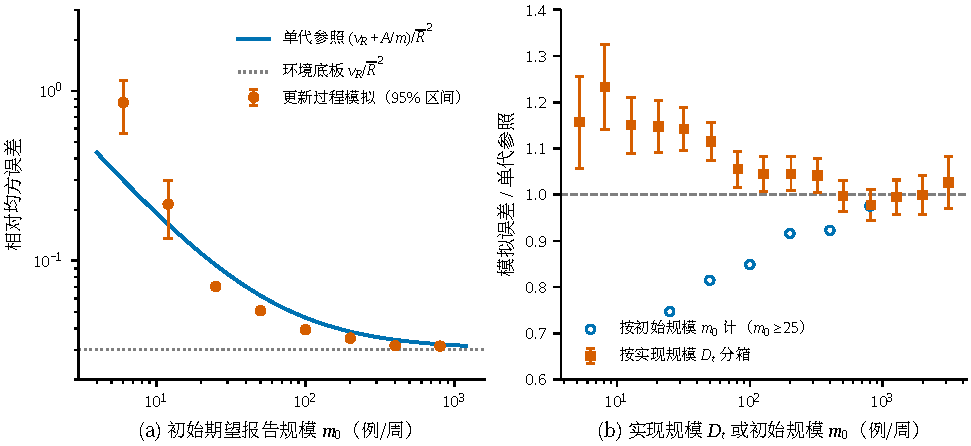
\includegraphics[width=\textwidth]{figures/fig_04_fig04_renewal_scale.pdf}
  \caption{更新过程仿真中的规模效应。每个初始规模 400 条轨迹，每条 26 个评价点，误差棒为 95\% 区间。(a) 增长统计量的相对均方误差随初始规模 $m_0$ 的变化，实线为单代参照曲线 $(v_R+A/m)/\overline{R}^2$，点线为环境底板。参照曲线不是误差下界。(b) 模拟误差与参照曲线之比：方块按实际规模 $D_t$ 分组，空心圆按初始规模 $m_0$（$m_0\geq25$）计算。}
  \label{fig:renewal}
\end{figure}
